% !TEX root = ../thesis.tex

\chapter{Conclusion}
\label{chap:conclusion}

\cleanchapterquote{“Knowledge is just opinion that you trust enough to act upon.}{Orson Scott Card}{(Children of the Mind)}


% ------------------------------------------------------------------------------

In Chapter~\ref{chap:theory} we saw multi-layer feedforward neural networks are universal approximators.
A sufficiently big fully-connected network could, theoretically, solve arbitrarily complex problems.
However, limited computational resources and training datasets make them unpractical for real-world tasks.
Deep neural networks are used instead, as they learn increasingly abstract notions instead of raw inputs and require much fewer learnable parameters.
Traditionally, pattern recognition algorithms required domain features to be carefully modeled by experts with knowledge on the field, but Deep Learning allows us to train neural networks to carry out feature engineering automatically for us.

In Chapter~\ref{chap:context} we reviewed how the feature extraction capabilities of deep neural networks consistently granted them the top positions in object recognition challenges.
It is remarkable how well we understand how to make neural networks work for object recognition, as they now rival human performance in many aspects, compared to how little we know about how they reason once they are trained.
To help understanding this, recently-developed techniques try to visualize internal representations of deep neural networks and have produced very intriguing images with with potential artistic implications.

In Chapter~\ref{chap:system} we presented the Neural Style algorithm and how it managed to solve a long-standing problem in artistic rendering: the separation of style and content.
Whereas the algorithm can produce visually compelling compositions of style and content from two different source images, it requires fine-tuning on a per-case basis.
This make us believe Neural Style fails to grasp the notion of ``aesthetics'', which is another unsolved problem in artistic rendering, often studied in \emph{algorithmic aesthetics}.

In Chapter~\ref{chap:applications} we surveyed a number of methods for improved style transfer and several other image transformation tasks that also rely on extracting visually perceptive features.
They all presenting superior performance than the state of the art in their respective field.

The separation of style and content had been a very difficult problem to solve because it depends on human non-objective perception of what is style and what is content in an artwork.
Formulating notions of ``aesthetics'' is a similarly complex problem, since we cannot formally define it and totally builds upon human perception.

Capturing subjective opinions is being currently researched.
At the time of writing this thesis, the Beauty.AI's First International Beauty Contest Judged by an Artificial Intelligence Jury \cite{YouthLaboratories} has taken place already.
Their promoters, supported by Nvidia and Microsoft among others, aim for teaching machines estimate human attractiveness by looking at the human face, relying for this on human biased perception.

In the light of the increasing interest in distilling inherently subjective features that are impractically to model formally, we find the study of aesthetics a relevant matter with practical applications.
Therefore, we believe the aesthetics of images could be similarly distilled and used for further improving artistic rendering techniques.


% ------------------------------------------------------------------------------

\section{Future Work}
\label{sec:conclusion:future}

We propose further work on building an aesthetics-driven deep neural network for style transfer.
The system would consist of two sub-networks: one for image transformations, and another for quality estimation.
The image transformation network, once trained, would produce perceptually compelling images.
For training it, an aesthetic estimation network would rate the perceptual quality of the generated images and this would be used as the loss function.

The first challenge is finding how to quantify the perceptual quality of an image.
That is, to model an inherently human subjective notion.
For that we propose a convolutional neural network (CNN) that should be trained for estimating aesthetics based on human opinion.
The network could be either trained from scratch or from one pre-trained for object recognition, applying transfer learning techniques \cite{Pan2010}, which basically allows the network to adjust to a slightly different task or domain.

In order to train the aesthetics estimation network we must have a sufficiently large and diverse training dataset of image-rating pairs.
We imagine a crowdsourcing platform with which to collect ratings from humans on artistic compositions.
People would be presented with two artistic images and they should decide which two of them appeal most to them.
This is currently being done similarly in DeepArt.io's for the artistic Turing test (\url{https://turing.deepart.io/}).

The artistic images people would be rating could be composed of images from three sources: 1) a repository of classical paintings, 2) user-submitted style transfer creations, and 3) randomly-generated style transfer creations.
This last source would be generated from the repository of classical paintings, some repository of photographs, and randomly chosen style transfer hyperparameters.
Including them is of particular interesting since it will result in a more diverse, less biased artistic creations, and once ratings are collected, therefore, in a more representative training dataset for the aesthetic estimation network.

Important considerations to be taken when deploying the crowdsourcing initiative would be: acquiring a sufficiently large initial repository of images to rate, incentives to invite people to contribute, user interaction design to keep the contribution process simple, and, finally, potential partnerships with industry for having access to computation facilities in which to run the initiative.

The second challenge, once the aesthetic estimation network had been trained, is designing and training the image transformation network.
We have identified three plausible directions thus far.

Our first intuition is using a CNN whose very last layer is the Neural Style algorithm, as is.
The image transformation network in this case would learn how the Neural Style hyperparameters must be adjusted to produce a perceptually compelling composition given a pair of source images.

Likewise, our second approach is having the Neural Style hyperparameters fixed to some relatively good values.
In this case, the image transformation network would instead learn how to correct the source images so that when processed by Neural Style the result would be appealing.

We anticipate two main problems with the previous approaches.
First, Neural Style is computationally expensive, as it requires of a backpropagation pass to produce the images, and relying on it would terribly slow down the learning process.
And second, we suspect reusing Neural Style as a black box layer would limit the meaning of the internal representations.

To circumvent this, and inspired by \cite{Johnson2016}'s approach, we would completely disregard Neural Style in the image transformation network.
The network would learn how to maximize the perceived quality of the composition for a fixed style and a given photograph in a simple feedforward pass.
The question is still open to see if the network could learn how to apply general style transfer given two images.
We conjecture, however, that, by using the aesthetics estimation network as part of the loss function, it can be possible.

We are certain, such a system will not only pose a versatile tool for artistic rendering, it will also be of great relevance to the advance in neuroscience.
Giving researchers a new way to look into how the creative process occurs in the human brain and what are the patterns in nature that elicit the notion of beauty in our minds.

\begin{figure}[!b]
  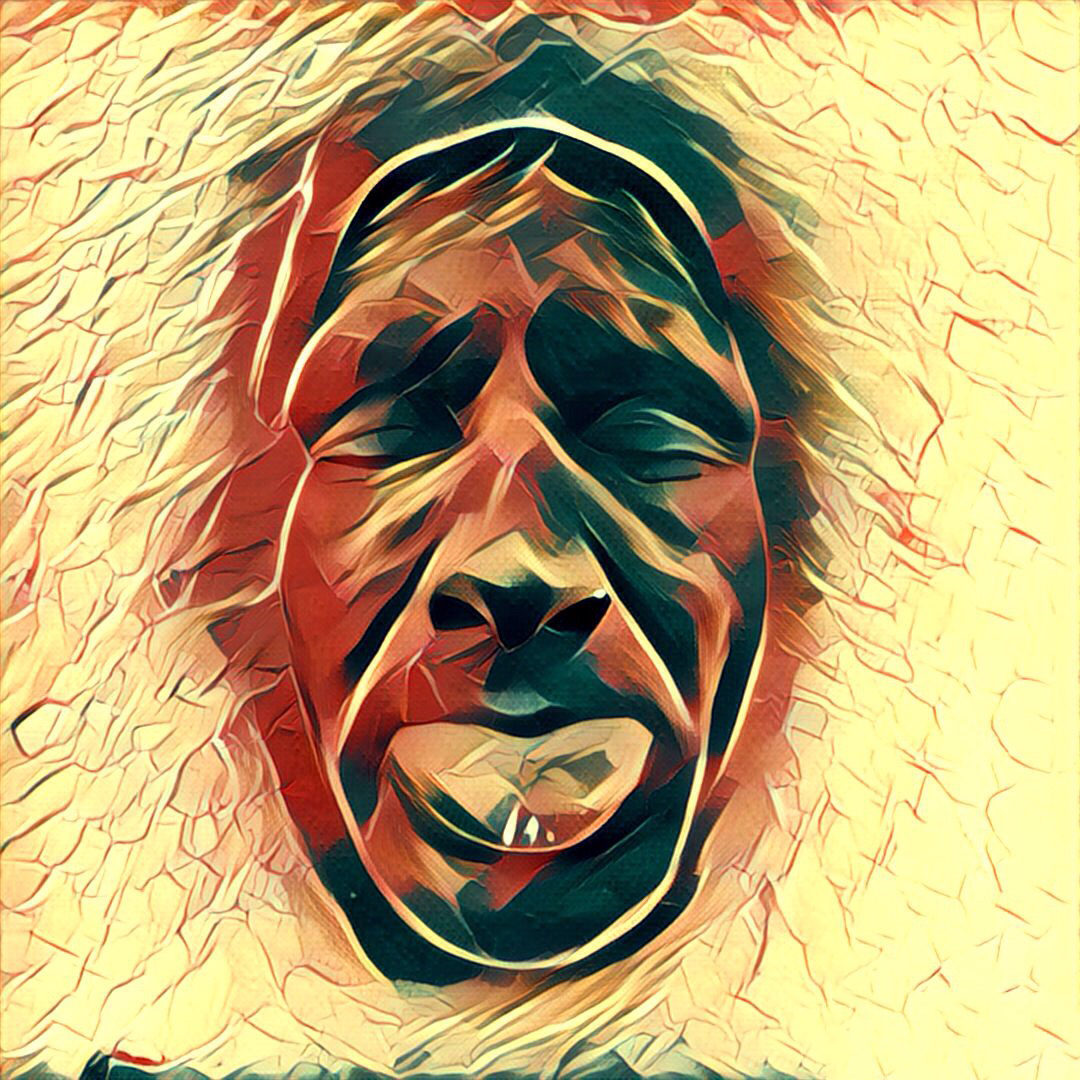
\includegraphics[width=\textwidth]{gfx/prisma}
\end{figure}
